\documentclass[tikz,border=5pt]{standalone}
\usepackage{amsmath}
\usetikzlibrary{arrows.meta,positioning,calc}

\begin{document}
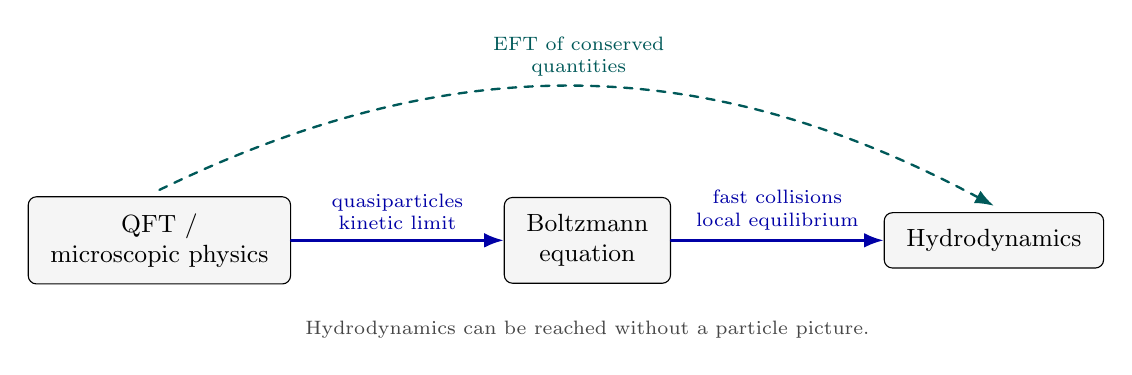
\begin{tikzpicture}[
    line cap=round,
    line join=round,
    >=Latex,
    node distance=2.7cm,
    box/.style={
        draw,
        rounded corners=3pt,
        fill=gray!8,
        inner xsep=8pt,
        inner ysep=6pt,
        align=center,
        font=\small
    },
    arrow/.style={->,line width=0.9pt,blue!65!black},
    direct/.style={->,line width=0.85pt,dashed,teal!70!black}
]

\node[box] (micro) {QFT /\\ microscopic physics};
\node[box,right=of micro] (boltzmann) {Boltzmann\\ equation};
\node[box,right=of boltzmann] (hydro) {Hydrodynamics};

\draw[arrow] (micro) -- node[above,font=\scriptsize,align=center] {quasiparticles\\ kinetic limit} (boltzmann);
\draw[arrow] (boltzmann) -- node[above,font=\scriptsize,align=center] {fast collisions\\ local equilibrium} (hydro);
\draw[direct] ($(micro.north)+(0,0.08)$) to[bend left=27]
    node[above,font=\scriptsize,align=center] {EFT of conserved\\ quantities}
    ($(hydro.north)+(0,0.08)$);

\node[font=\scriptsize,align=center,text=gray!55!black] at ($(boltzmann.south)+(0,-0.58)$)
    {Hydrodynamics can be reached without a particle picture.};

\end{tikzpicture}
\end{document}
